\documentclass[10pt, oneside]{article} 
\usepackage{amsmath, amsthm, amssymb, calrsfs, wasysym, verbatim, bbm, color, graphics, geometry}
\usepackage[colorlinks=true, linkcolor=blue, urlcolor=blue, citecolor=blue]{hyperref} % Customize hyperref
\usepackage{csquotes} % For the \enquote command
\usepackage[dvipsnames]{xcolor} % For colored text
\usepackage{tcolorbox} % For custom boxes
\usepackage{multicol}
\usepackage{float}

\usepackage{tikz}
\usetikzlibrary{arrows.meta, decorations.markings}
\tikzset{
    vector/.style={thick,->},
    angle/.style={thin, red},
    angle label/.style={font=\small, red},
}

\usepackage{multicol}

\usepackage{csquotes}

\newtheorem{theorem}{Theorem}
\newtheorem*{theorem*}{Theorem}

\theoremstyle{remark}
\newtheorem*{own_abstract}{Abstract}
\newtheorem*{proofsketch}{Proof Sketch}

% Define the new command for boxed notes
\newcommand{\myBoxedNote}[1]{%
  \hspace{40pt} \boxed{\textbf{Sidenote: } #1}%
}

% counter for definitions
\newcounter{definition}
% Define the new environment for definitions
\newtcolorbox{myDef}[1][]{
  colback=gray!10!white, colframe=gray!80!black, fonttitle=\bfseries,
  title=Definition \thedefinition\ifstrempty{#1}{}{ (#1)},
  rounded corners, before upper={\stepcounter{definition}}
}

% counter for theorems
\newcounter{theoremCounter}

% define the new environment for theorems
\newtcolorbox{myTheo}[1][]{
  colback=red!10!white, colframe=red!50!black, fonttitle=\bfseries,
  title=Theorem \thetheoremCounter\ifstrempty{#1}{}{ (#1)},
  rounded corners, before upper={\stepcounter{theoremCounter}}
}

\newcounter{claimCounter}
\newtcolorbox{myClaim}[1][]{
  colback=white, colframe=black, fonttitle=\bfseries,
  title=Claim \theclaimCounter\ifstrempty{#1}{}{ (#1)},
  rounded corners, before upper={\stepcounter{claimCounter}}
}

\geometry{tmargin=.75in, bmargin=.75in, lmargin=.75in, rmargin = .75in}  

\newtheorem{thm}{Theorem}
\newtheorem{defn}{Definition}
\newtheorem{conv}{Convention}
\newtheorem{rem}{Remark}
\newtheorem{lem}{Lemma}
\newtheorem{cor}{Corollary}

\title{\textbf{Documentation} \\ Mini Games using Arduino}
\author{Fabian Stiewe}
\date{Academic Year 2024-2025}

\begin{document}

\maketitle
\tableofcontents

\newpage

\section{Introduction}
This document is a collection of all the information needed for the project documentation. It is a summary of the project and includes all the necessary information for the project.

\vspace{1em}

The file titled \enquote{Project\_From.pdf} provides more general information about the school, year, learning objectives, and other relevant details, filling in the gaps in this document.

\section{Project Description}

My project is about creating different \enquote{MiniGames} with the Arduino Uno. The games are simple and fun to play. The games are implemented using the Arduino Uno and the components mentioned below. The games are TicTacToe, SimonSays, and any other game the students come up with.

\subsection{General Framework}
In all projects only the following components are mandatory, depending on the project the students choose, additional components may be needed (\textit{see \ref{any_other_game}}):
\begin{itemize}
  \item Arduino Uno
  \item Breadboard
  \item Jumper Wires
\end{itemize}

\subsection{TicTacToe}
TicTacToe is a two player game, where the players take turns to place their symbol on the board. The board is a 3x3 grid. The first player to get three of their symbols in a row, column or diagonal wins the game. The game ends in a draw if all the fields are filled and no player has three of their symbols in a row, column or diagonal.

\subsubsection{Additional components}
For my implementation of the TicTacToe game I used the following additional components:
\begin{itemize}
  \item LED
  \begin{itemize}
    \item Green LED
    \item Red LED
    \item Yellow LED
    \item (Blue LED)
  \end{itemize}
  \item Buzzer
  \item OLED Display
  \item Keypad
  \item Resistors (220$\Omega$)
  \item Diverse cables
\end{itemize}
You can see the circuit diagram in Figure \ref{fig:circuit_diagram} and the circuit blocks in Figure \ref{fig:circuit_blocks}.

\subsubsection{Code}
The sketch operates in the following manner: 

\begin{itemize}
    \item Initially, you \textbf{initialize} the \textit{OLED Display}, \textit{Keypad}, \textit{LEDs}, and \textit{Buzzer} within the \texttt{setup()} function. 
    \item Subsequently, you create various \textbf{variables} for the game, such as the \texttt{board}, the \texttt{current player}, the \texttt{winner}, and so on.
\end{itemize}

\noindent Firstly, you draw a \textbf{Menu screen} to introduce the user and prompt them to \textbf{press \texttt{1} to commence the game}. Upon pressing \texttt{1}, the game commences, the \textbf{GameStatus} undergoes a change, and the user is permitted to play.

\noindent During the game:
\begin{itemize}
    \item The \textbf{board} is drawn, and it also displays the standings.
    \item The user can \textbf{press a button} from $1$ to $9$ on the keypad to \textbf{place their symbol on the board}.
    \item The game \textbf{verifies the validity of the move}, \textbf{updates the board}, and \textbf{checks if the current player has achieved victory}.
\end{itemize}

\noindent If the current player has \textbf{won}, the game concludes, and the \textbf{winner is displayed}. If the game ends in a \textbf{draw}, the game concludes, and the \textbf{draw is displayed}. If neither of these conditions is met, the \textbf{game continues}, and the \textbf{player’s turn changes}.

\subsubsection{Programming Guide}
\begin{enumerate}
  \item Initialize the \textit{OLED Display}
  \begin{itemize}
    \item \href{https://www.az-delivery.de/en/collections/kostenlose-e-books}{Free E-Book for OLED Display documentation}
  \end{itemize}
  \item Initialize the \textit{Keypad}
  \begin{itemize}
    \item \href{https://www.az-delivery.de/en/collections/kostenlose-e-books}{Free E-Book for Keypad documentation}
  \end{itemize}
  \item Initialize the \textit{Buzzer}
  \item Initialize the \textit{LEDs} (Green, Red, Yellow, Blue)
  \item Inside the \texttt{setup()} function, initialize the \textit{OLED Display}, \textit{Keypad}, \textit{Buzzer}, and \textit{LEDs}.
  \item Create an \texttt{enum} for different game states.
  \item Create the following variables for the game:
  \begin{itemize}
    \item startingGame - Melody, note-duration and length of the melody
    \item player\textbf{0} - move-note, move-note-duration
    \item player\textbf{1} - move-note, move-note-duration
    \item win - Melody, note-duration and length of the melody
    \item draw - Melody, note-duration and length of the melody
    \item bool - if the win or draw melody should be played
    \item int - current player, player\textbf{0} score, player\textbf{1} score, current move
    \item char - board[3][3][2] 
    \begin{itemize}
      \item 3x3 board 
      \item Each field is " ", "X" or "O"
    \end{itemize}
    \item helper variables for the OLED Display for a more fluent gameplay - bool boardDrawn, bool setupGame, int counterLastMove, int counterBoardDrawnFinal
  \end{itemize}
  \item Create the different loops for the game, for the different game states.
  \item Function to loop the Menu
  \item Create a function to draw the Menu
  \item Create a function to get the user input inside the menu
  \item Function to loop the Games
  \item Create a function to draw the TicTacToe board
  \item Create a function to check if the current player has won or if the game ended in a draw
  \begin{itemize}
    \item Check winner by checking each row, col and diagonal
    \item Check if the board is full for draw
    \item \textbf{Note:} Create one function for Winner checking and one function for Draw checking
    \item If either of these conditions is met, the game concludes, the winner or draw is displayed and the game status changes
  \end{itemize}
  \item Create a function to get the user input inside the game
  \begin{itemize}
    \item Get a number from the keypad
    \item Check if the number is between 1 and 9
    \item Check if the field is empty
    \item Update the board (using a helper function)
    \item Increase the number of moves
    \item Play the move sound for the current player
    \item Switch the current player
  \end{itemize}
  \item Create a function to update the board
  \item Create a function to display the current standings
  \item Create a function to play the melody
  \item Create a function to draw the game over screen
  \item Create a function to get the user input inside the game over screen
  \item After the game reset everything except:
  \begin{itemize}
    \item player\textbf{0} score, player\textbf{1} score
    \item current player
  \end{itemize}
\end{enumerate}

\subsection{Simon Says}
SimonSays is a game where the player has to repeat a sequence of colors and sounds. The sequence starts with one color and its corresponding sound and gets longer each round by $1$. The player has to repeat the sequence correctly to continue to the next round. If the player makes a mistake the game ends.

\subsubsection{Additional components}
For my implementation of the TicTacToe game I used the following additional components:
\begin{itemize}
  \item LED
  \begin{itemize}
    \item Green LED
    \item Red LED
    \item Yellow LED
    \item (Blue LED)
  \end{itemize}
  \item Buzzer
  \item OLED Display
  \item Keypad
  \item Resistors (220$\Omega$)
  \item Diverse cables
\end{itemize}
You can see the circuit diagram in Figure \ref{fig:circuit_diagram} and the circuit blocks in Figure \ref{fig:circuit_blocks}.

\subsubsection{Code}
The sketch operates in the following manner:

\begin{itemize}
  \item Initially, you \textbf{initialize} the \textit{OLED Display}, \textit{Keypad}, \textit{LEDs}, and \textit{Buzzer} within the \texttt{setup()} function. 
  \item Subsequently, you create various \textbf{variables} for the game, such as the \texttt{sequence}, the \texttt{player sequence}, the \texttt{current round}, and so on.
\end{itemize}

\noindent Firstly, you draw a \textbf{Menu screen} to introduce the user and prompt them to \textbf{press \texttt{1} to commence the game}. Upon pressing \texttt{1}, the game commences, the \textbf{GameStatus} undergoes a change, and the user is permitted to play.

\noindent During the game:
\begin{itemize}
  \item The game \textbf{displays} to \enquote{WATCH} and \textbf{plays the sequence}.
  \item The user has to \textbf{repeat the sequence} by \textbf{pressing the corresponding buttons} on the keypad, which are from $0$ to $3$.
  \item The game \textbf{verifies the correctness of the sequence}.
  \item If the sequence is correct, the game \textbf{goes into the round round} and randomly creates a new sequence, which is longer by $1$.
  \item If the sequence is incorrect, the game \textbf{ends}, and the \textbf{correct sequence} will be displayed.
\end{itemize}

\subsection{Programming Guide}
\subsubsection{Programming Guide}
\begin{enumerate}
  \item Initialize the \textit{OLED Display}
  \begin{itemize}
    \item \href{https://www.az-delivery.de/en/collections/kostenlose-e-books}{Free E-Book for OLED Display documentation}
  \end{itemize}
  \item Initialize the \textit{Keypad}
  \begin{itemize}
    \item \href{https://www.az-delivery.de/en/collections/kostenlose-e-books}{Free E-Book for Keypad documentation}
  \end{itemize}
  \item Initialize the \textit{Buzzer}
  \item Initialize the \textit{LEDs} (Green, Red, Yellow, Blue)
  \item Inside the \texttt{setup()} function, initialize the \textit{OLED Display}, \textit{Keypad}, \textit{Buzzer}, and \textit{LEDs}.
  \item Create an \texttt{enum} for different game states.
  \item Create the following variables for the game:
  \begin{itemize}
    \item level - current level
    \item charLightSequence[] - sequence of lights
    \item Helper variables for the OLED Display for a more fluent gameplay - int counterShowLightShow, int counterAskForUserInput, int counterShowCorrect \textit{(Those may not be necessary!)}
  \end{itemize}
  \item Create the different loops for the game, for the different game states.
  \item Starting with the loopPhaseInstructions
  \begin{itemize}
    \item Display the name of the game
    \item Ask for any key to start the game
    \item Create a function to get the user input, to start the game
  \end{itemize}
  \item Create a function to loop lightShow
  \begin{itemize}
    \item Write on the OLED Display "WATCH"
    \item Wait for a short time, so WATCH is correctly displayed
    \item Play the sequence of lights and corresponding sounds
    \begin{itemize}
      \item Get a random number between 0 and 3
      \item Store this number so the user input can be compared to it
      \item Turn on the corresponding LED for a short time and play the corresponding sound
      \item Delay between the lights and sounds
      \item Change the game phase to user input
    \end{itemize}
  \end{itemize}
  \item Create a function to loop user input
  \begin{itemize}
    \item Write on the OLED Display "REPEAT" (or equivalent)
    \item Wait for a short time, so REPEAT is correctly displayed
    \item Get the user input
    \begin{itemize}
      \item Get a number from the keypad
      \item Check if the number is between 0 and 3, if not, ignore the input and wait for the next input \textbf{This is not an error!}
      \item If the number is between 0 and 3
      \begin{itemize}
        \item Check if the user input is correct
        \item Do this by comparing the user input with the light sequence
        \item Play the corresponding sound and turn on the corresponding LED for a short time
      \end{itemize}
      \item If all inputs are correct, change the game phase to correct
      \begin{itemize}
        \item Show a success message
        \item Wait a short time
        \item Increase the level
        \item Go back to the lightShow phase
      \end{itemize}
      \item If the input is incorrect, change the game phase to wrong input
      \begin{itemize}
        \item Show a failure message 
        \item Show the correct sequence
        \item Wait a short time
        \item Ask for any key to start the game again
      \end{itemize}
    \end{itemize}
  \end{itemize}
\end{enumerate}

\subsection{Any other game}
\label{any_other_game}
Students are encouraged to come up with their own game ideas and implement them. The game should be simple and fun to play. The game should also be implemented using the Arduino Uno and the components mentioned above. 

\subsubsection{Additional components}
Students are free to use any additional components they wish, but it’s recommended to consult the teacher first so that the teacher can provide guidance and assistance if necessary.

\section{Circuit Diagram}
\begin{figure}[H]
  \begin{center}
    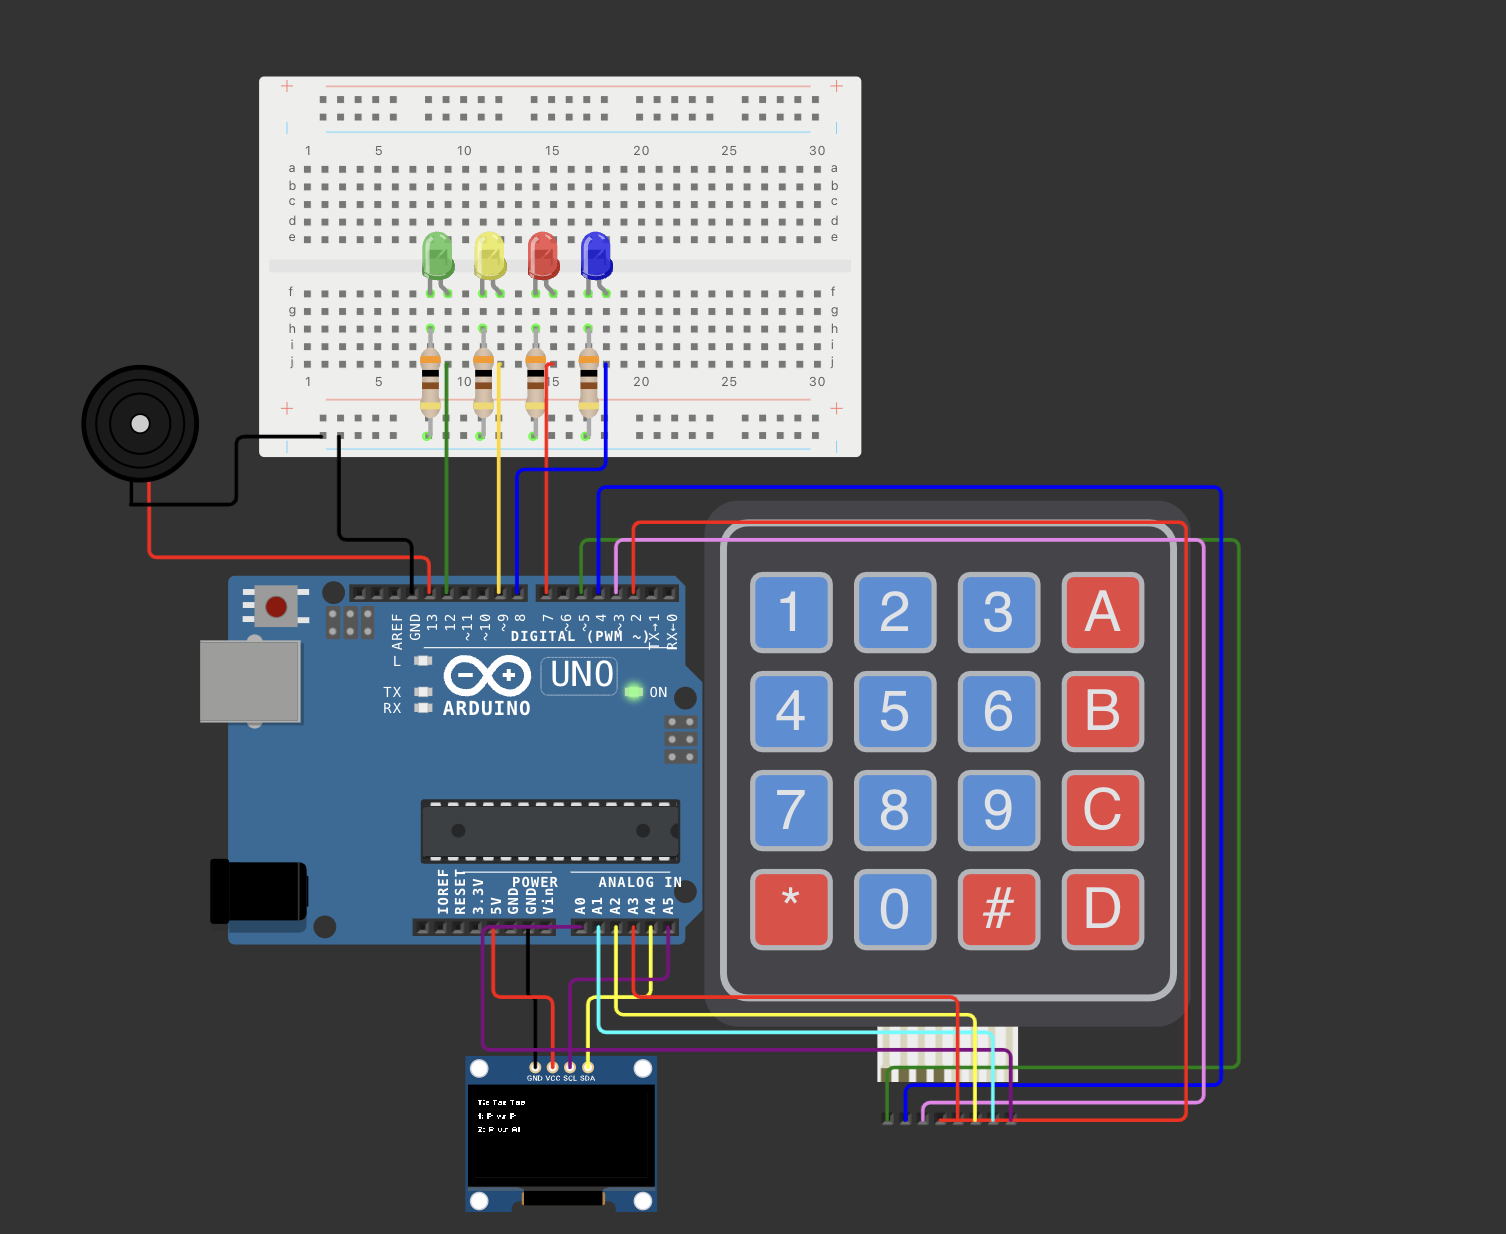
\includegraphics[width=0.7\textwidth]{CircuitDiagram.png}
  \end{center}
  \caption{Circuit Diagram created using Wokwi}
  \label{fig:circuit_diagram}
\end{figure}

\section{Circuit Blocks}
\begin{figure}[H]
  \begin{center}
    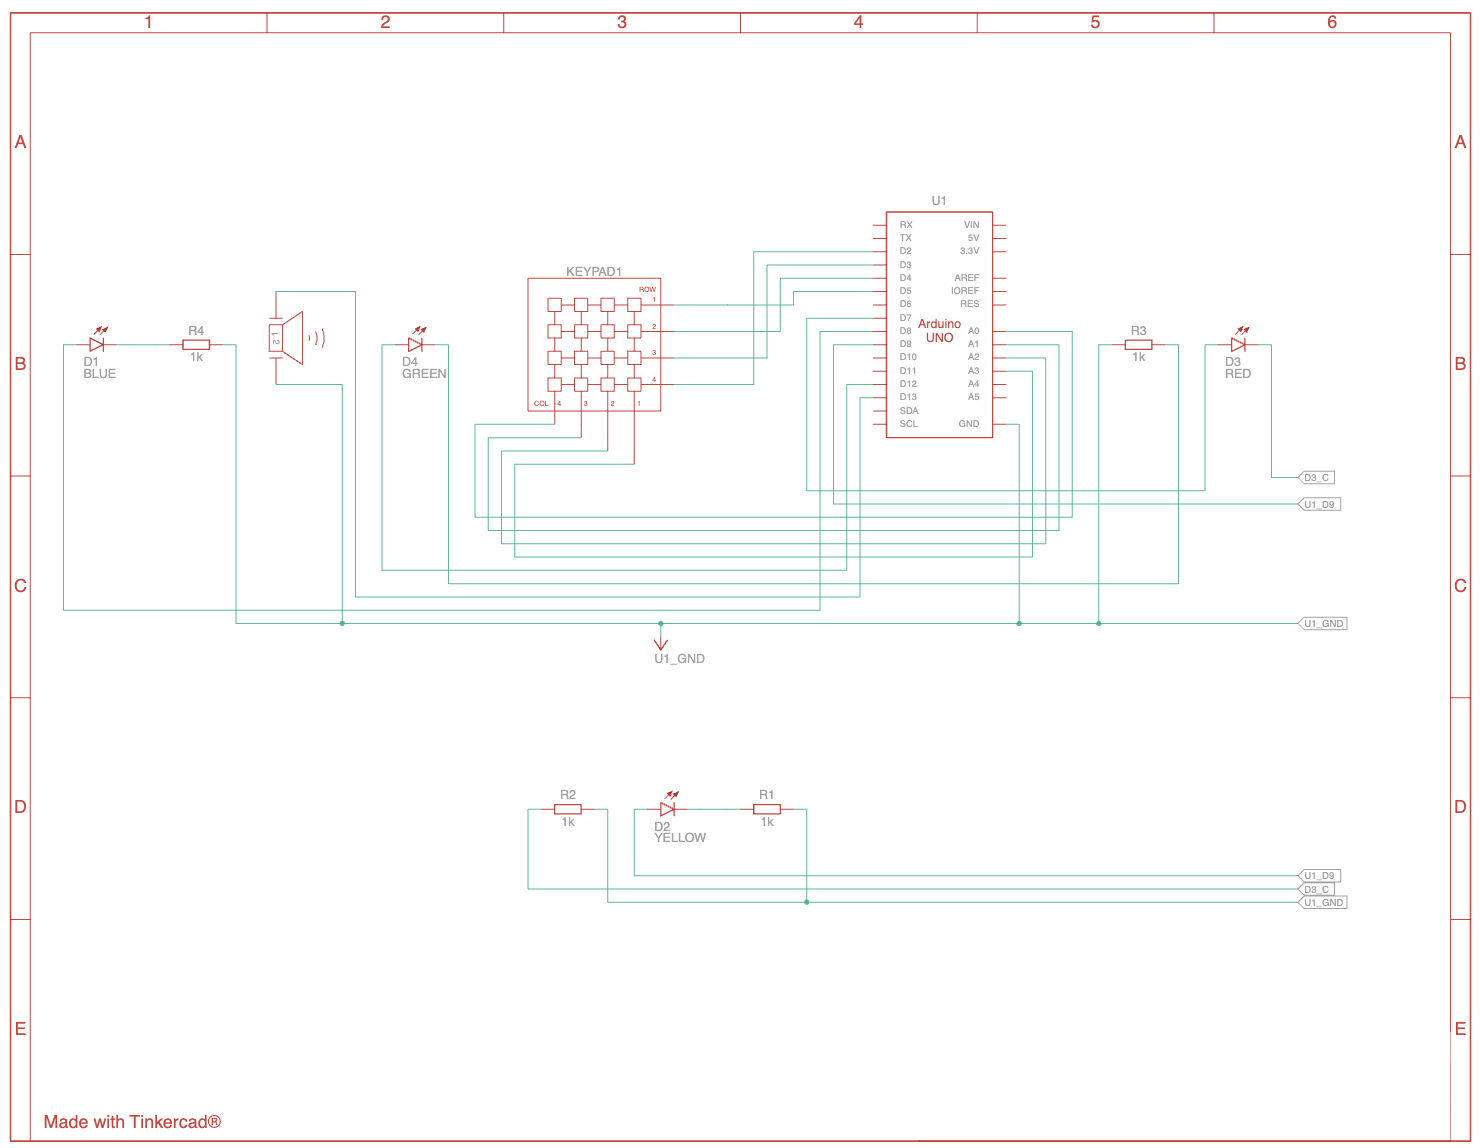
\includegraphics[width=0.7\textwidth]{CircuitBlocks.png}
  \end{center}
  \caption{Circuit Blocks created using Tinkercad}
  \label{fig:circuit_blocks}
\end{figure}
\textit{Note: This is unfortunately not complete, because the OLED Display is not available in Tinkercad.}

\end{document}